\documentclass[10pt]{article}

\usepackage{tex-assets/sbc-template} 
\usepackage{graphicx,url}
\usepackage{url}
\usepackage[utf8]{inputenc} 
\usepackage[T1]{fontenc}
\usepackage[normalem]{ulem}
\usepackage[hidelinks]{hyperref}

\usepackage[square,authoryear]{natbib}
\usepackage{amssymb} 
\usepackage{mathalfa} 
\usepackage{algorithm} 
\usepackage{algpseudocode} 
\usepackage[table]{xcolor}
\usepackage{array}
\usepackage{titlesec}
\usepackage{mdframed}
\usepackage{listings}

\usepackage{amsmath} 
\usepackage{booktabs}

\usepackage{indentfirst}
\usepackage{wrapfig}

\urlstyle{same}

\newcolumntype{L}[1]{>{\raggedright\let\newline\\\arraybackslash\hspace{0pt}}m{#1}}
\newcolumntype{C}[1]{>{\centering\let\newline\\\arraybackslash\hspace{0pt}}m{#1}}
\newcolumntype{R}[1]{>{\raggedleft\let\newline\\\arraybackslash\hspace{0pt}}m{#1}}

\newcommand\Tstrut{\rule{0pt}{2.6ex}} 
\newcommand\Bstrut{\rule[-0.9ex]{0pt}{0pt}} 
\newcommand{\scell}[2][c]{\begin{tabular}[#1]{@{}c@{}}#2\end{tabular}}

\usepackage[nolist,nohyperlinks]{acronym}

\newcommand{\baseline}[0]{\textit{\textbf{baseline design}}}
\newcommand{\alternative}[0]{\textit{\textbf{alternative design}}}

\title{Lab 1: Iterative Multiplier}

\author{Joseph Whelan (jfw225@cornell.edu)}

\address{ECE 4750: Computer Architecture, Fall 2022, Cornell University}



\begin{document} 
	
	\maketitle
	
	\section{Introduction}
	\label{sec:introduction}

	By the end of this semester, we will have implemented a modern shared-memory multicore system. The purpose of this lab was to build one of the fundamental components of this system in addition to developing an efficient workflow and familiarity with the framework with which we have been provided. More specifically, we built two versions of an iterative 32-bit multiplier that are capable of multiplying two 32-bit numbers in at most 35 clock cycles. 
	
	The \baseline~ takes exactly 35 clock cycles to complete its multiplication. Additionally, the \baseline ~comprises a \textit{datapath module} (Figure \ref{fig:base_dpath}) which produces the output message by moving the input data through "various arithmetic blocks, muxes, and registers" and the \textit{control module} (Figure \ref{fig:base_ctrl}) which manipulates the control signals (highlighted in blue in Figure \ref{fig:base_dpath}) \citep*{lab_handout}. The second version, which we refer to as the \alternative, builds on the architecture of the \baseline~ with a couple of minor optimizations that reduces the number of clock cycles required to complete the multiplication. 
	
	\section{Alternative Design}
	\label{sec:alt_design}

	\noindent Before we can discuss the RTL implementation of either design, we must first understand the algorithm that is being implemented.

	\subsection{The Iterative Multiplier Algorithm}
	\label{sec:imul_algo}

	\begin{wrapfigure}{r}{7.5cm}
		\includegraphics[width=0.5\textwidth]{figures/imul-base-code-py.png} 
		\caption{Python Implementation of the Base Iterative Multiplication Algorithm}
		\label{fig:base_code_py}
	\end{wrapfigure} 

	\noindent On the right, we have a code snippet of an implementation of the iterative multiplication algorithm in Python (Figure \ref{fig:base_code_py}). The function \texttt{imul\_base} takes two 32-bit integers as parameters $a,b$. After initializing the output value to zero, the function iterates through each bit of $b$ and adds $a$ to the output if the least significant bit of $b$ is set. The function then shifts $a$ to the left by one bit, shifts $b$ to the right by one bit, and repeats this process until $b$ is zero. This can effectively by thought of as the summation of partial-products given by
	$$\sum_{i=0}^{31} a \cdot 2^i \cdot b_i,$$
	where $b_i$ is the $i$-th bit of $b$.

	\pagebreak

	\noindent Notice that this loops 32 times but only performs an addition operation when $b_i\not=0$ which occurs $N$ times, where $N$ is given by 
	$$32\geq N = \sum_{i=0}^{31} b_i.$$
	Thus, there are $32-N$ clock cycles that are wasted. This is the motivation for the \alternative.

	\begin{wrapfigure}{l}{7.5cm}
		\includegraphics[width=0.5\textwidth]{figures/imul-alt-code-py.png} 
		\caption{Python Implementation of the Alternative Iterative Multiplication Algorithm}
		\label{fig:alt_code_py}
	\end{wrapfigure} 

	\noindent On the left, we have a code snippet of an implementation of the alternative iterative multiplication algorithm in Python (Figure \ref{fig:alt_code_py}). The function \texttt{imul\_alt} takes two 32-bit integers as parameters $a,b$. The alternative function first initializes a counter to zero in addition to the output value. Like before, \texttt{imul\_alt} loops through the bits of $a$ and $b$, but instead of shifting by one at each iteration, it does something a little different.
	
	\noindent We observed previously that we waste a clock cycle when $b_i=0$. The alternative algorithm takes advantage of this by counting the number of trailing zeros in $b$ and shifting each value by that amount. This allows us to skip over the clock cycles that would have been wasted and only perform the addition operation when $b_i\not=0$. One important note is that in software, the naive method of counting the trailing zeros in $b$ has a time complexity of $O(n)$ where $n$ is the number of bits in $b$. However, we can use hardware to count $b$'s trailing zeros in $O(1)$ time which is what we do in the \alternative.

	\subsection{Functional-Level Description}
	\label{sec:alt_fld}

	Both the \baseline~ and \alternative~ can be described at the functional-level by Figure \ref{fig:imul_fl_design}

	\begin{figure}[!ht]
		\centering
		\includegraphics[width=0.7\textwidth]{figures/imul-design.png}
		\caption{Functional-Level Implementation of the Integer Multiplier}
		\label{fig:imul_fl_design}
		\citep*{lab_handout}
	\end{figure}

	where each of the I/O lines is explained in Table \ref{tab:imul_fl_params}.

	\begin{table}[!ht]
		\centering
		\begin{tabular}{|| c | c | c | p{80mm} ||} 
			\hline
			I/O Lines & Type & Bit Width & Description \\ [0.5ex] 
			\hline\hline
			\texttt{istream\_msg} & Input & 64 & Concatenation of two 32-bit integers $a,b$ where the most significant 32 bits correspond to $a$ and the least significant 32 bits correspond to $b$. \\
			\hline
			\texttt{istream\_val} & Input & 1 & Validation bit for \texttt{istream\_msg}. Setting this signal indicates to the multiplier \texttt{istream\_msg} is valid and that it can start with the multiplication. \\
			\hline
			\texttt{istream\_rdy} & Output & 1 & Ready bit for \texttt{istream\_msg}. If this signal is set, then the multiplier is ready to receive new input data. \\
			\hline
			\texttt{ostream\_msg} & Output & 32 & The output of the multiplication, or rather $a\cdot b$. \\
			\hline
			\texttt{ostream\_val} & Output & 1 & Validation bit for \texttt{ostream\_msg}. If this signal is set, then the value of \texttt{ostream\_msg} is valid for the given input. \\
			\hline
			\texttt{ostream\_rdy} & Input & 1 & Ready bit for \texttt{ostream\_msg}. If this signal is set, then the multiplier will write output data to \texttt{ostream\_msg}. \\ [1ex] 
			\hline
		\end{tabular}
		\caption{\label{tab:imul_fl_params}Input/Output Parameters for the Functional-Level Implementation of the Iterative Multiplier}
	\end{table}

	\subsection{RTL Implementation}
	\label{sec:alt_rtl}

	Both the \baseline~ and \alternative~ implement the functional-level design described by Figure \ref{fig:imul_fl_design} with a similar architecture. The designs implement the algorithms discussed in Section \ref{sec:imul_algo} using two co-designed modules: the datapath (design show in Figure \ref{fig:base_dpath}) and the control unit (FSM shown in Figure \ref{fig:base_ctrl}).

	\begin{figure}[!ht]
		\centering
		\begin{minipage}{0.5\textwidth}
			\centering
			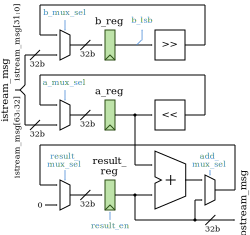
\includegraphics[width=0.9\textwidth]{figures/imul-base-dpath.png}
			\caption{Datapath for Fixed-Latency Iterative Integer Multiplier}
			\label{fig:base_dpath}
			\citep*{lab_handout}
		\end{minipage}\hfill
		\begin{minipage}{0.5\textwidth}
			\centering
			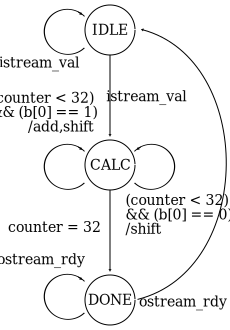
\includegraphics[width=0.6\textwidth]{figures/imul-base-ctrl.png} 
			\caption{Control FSM for Fixed-Latency Iterative Multiplier}
			\label{fig:base_ctrl}
			\citep*{lab_handout}
		\end{minipage}
	\end{figure}
	
	As shown in Figure \ref{fig:base_ctrl}, can be modeled as a finite-state machine with three state: \textbf{IDLE}, \textbf{CALC}, \textbf{DONE}. In each of these states, the control unit communicates with the datapath module using the blue-highlighted signals in Figure \ref{fig:base_dpath} depending on the value of the input signals.

	Inside of the datapath module, we separate \texttt{istream\_msg} into two 32-bit integers $a$ and $b$ with the goal of storing their product in an output that we'll refer to as $c$. Without loss of generality (with respect to $a,b,c$ and $<<,>>,+$), there is a mux that separates $a$ from the intermediate value that is manipulated during computation which we will call $a'$. The mux enables the control unit to determine if $a'=a$ or $a'=a'\cdot2^\Delta$ with the signal \texttt{a\_mux\_sel}, where $\Delta$ is number of bits by which we shift $a'$. More specifically, the control unit waits in the \textbf{IDLE} state for \texttt{istream\_val} to be set--at which point, the control unit enters the \textbf{CALC} state and starts the computation by setting \texttt{a\_mux\_sel} to initialize $a'=a$ and load it into a register.
	
	As a quick aside, the usage of a validation signal and internal register in this way yields a highly flexible and modular system. Since the datapath loads $a'$ into a register, the multiplier is independent from the initial input data $a$ after one cycle of \texttt{istream\_val} being set. Thus, the system that encompasses the multiplier is free to change the value of \texttt{istream\_msg} without affecting the multiplier's computation. This allows for the encompassing system to be spatially efficient with data storage.

	Once the computation begins, the control unit starts to keep track of how many cycles it has spent performing the multiplication with a simple counter. As the counter increments toward 32 with every cycle, the datapath module updates the signal tracking the least significant bit of $b$ with the signal \texttt{b\_lsb}. The control unit then uses this signal to determine if the current value of $a'$ should be added to $c'$. More specifically, if the least significant bit of $b'$ is 1, the control unit sets the value of \texttt{add\_mux\_sel} which instructs the datapath module to store the output of the 32-bit adder in the intermediate result register (i.e. $c'=c'+a'$). Once the counter has reached 32, the control unit knows that the multiplication is complete. It then enters the \textbf{DONE} state and lowers the value of \texttt{result\_en} to ensure that the correct output is not overwritten on subsequent cycles. Furthermore, the control unit waits in the \textbf{DONE} state until the encompassing system raises the value of \texttt{ostream\_rdy} before returning to the \textbf{IDLE} state.

	Adding on to what we discussed in an earlier paragraph, the usage of the ready signal and the result register further improve the flexibility and modularity of the system. Suppose that we don't need the output of the multiplier right away. The system that instantiates the multiplier can use \texttt{ostream\_msg} for other tasks until the multiplier finishes its computation. At which point, the instantiating system can raise \texttt{ostream\_rdy} which instructs the multiplier to write the output data to \texttt{ostream\_msg}. This modularity enables the encapsulating system to be allocatively efficient with all of its resources. 

	\subsection{Modifications for the Alternative Design}
	\label{sec:alt_mods}

	Going from an RTL implementation of the \baseline~ to the \alternative~ is very similar to going from the base implementation in Python (Figure \ref{fig:base_code_py}) to the alternative implementation in Python (Figure \ref{fig:alt_code_py}). If we look at the two Python implementations, the only difference is that we count the number of trailing zeros in $b'$ instead of only looking at the least significant bit and then shifting each of the intermediate values accordingly.
	
	\begin{wrapfigure}{r}{7.5cm}
		\includegraphics[width=0.5\textwidth]{figures/shift-delta-code.png} 
		\caption{Excerpt of the Alternative Control Unit Implementation Showing Shift $\Delta$ Calculation}
		\label{fig:shift_delta_code}
	\end{wrapfigure} 

	\noindent So we'll start with the first problem: counting the number of trailing zeros in $b'$. In Python, we were able to simply look at each trailing bit one-by-one. As I mentioned earlier, this is not computationally efficient and is actually worse than the base implementation because the count function runs in $O(n)$ time. However, we can build hardware that accomplishes this in $O(1)$ time. Taking a look at Figure \ref{fig:shift_delta_code}, we computed number of trailing zeros in $b'$ using a ternary statement that evaluates to some number $z$ if and only if the last $z$ bits in $b'$ are zero. Note that when this Verilog code is synthesized, it will be converted to some hardware equivalent to a mux. We did this by modifying \texttt{b\_lsb} to be a signal of size 4 instead of 1. Our choice for the number $4$ is arbitrary and can be changed to any number between $1$ and $32$. The larger the number, the more efficient the multiplier will be. However, there is a trade-off between efficiency and hardware utilization.

	The second problem is applying the shift $\Delta$ to $a'$. If we look back at Figure \ref{fig:alt_code_py} we not only applied the shift $\Delta$ to $a',b'$ but also to the counter. Thus, we use the shift $\Delta$ to update the counter inside of the control unit, and we add \texttt{shift\_delta} as an input to the datapath module. The datapath module then uses this signal to shift $a'$ and $b'$ by $\Delta$ bits.
	
	\section{Testing Strategy}
	\label{sec:testing_strategy}

	In order to ensure that our iterative multipliers were correct, it was imperative that we built a test suite that was as robust as possible. We did this by utilizing Python and \texttt{pymtl3} to build as massive test suite, and then added detailed information to the line tracing section for ad-hoc testing.

	We have found that it is extremely important to implement a strong testing infrastructure before implementing any sort of architecture. This is why we built our test suite before we started writing any Verilog. The naive approach to testing this multiplier would have been to ensure that it worked for every possible 32-bit number. Obviously, this is not feasible, so we instead tried to think about several test groups that may provide a basis for the problem space as a whole. For example, testing large positive numbers versus numbers whose more significant bits were masked. From this mindset, we choose a set of features that we felt could adequately map the problem space. More specifically, we chose to test the following features:
	\begin{itemize}
		\item Size: large vs. small
		\item Sign: positive vs. negative
		\item Parity: even vs. odd
		\item Masking: lower 16 bits masked, upper 16 bits masked, upper 8 and lower 8 bits masked, middle 16 bits masked
		\item Density: dense vs. sparse
		\item Special cases:
		\begin{itemize}
			\item all permutations of $-1,0,1$
			\item randomizing the number of zeros in the four most significant bits
		\end{itemize}
	\end{itemize}

	Before we proceed, we want to mention the importance of the last special test case: randomizing the number of zeros in the four most significant bits. Since we arbitrarily chose to look at the 4 least significant bits of $b'$, we anticipated that the shift $\Delta$ might cause a problem in the $28-32$ bit band for the counter or the other variables. And sure enough, there was. For our base implementation, we used the \texttt{vc\_BasicCounter} module that was provided to us. This module takes as a parameter (compile-time) the bit width of the counter. Since our counter could only go up to $32$, we set the bit width to $5$. However, this caused a problem whenever the counter value was at $v>=28$ and $\Delta>=32-v$. Since we chose a counter bit width of $5$, the counter would overflow and wrap around to $0$. This caused the multiplier to loop forever with certain inputs. To fix this, we simply changed the counter bit width to $6$ and the problem was solved. And fortunately, it did not take long to debug this problem because of the last special test case.

	Back to testing as a whole, we took each feature that we identified and generated many numbers that corresponded to that feature. Doing this yielded about $2,500$ test cases. We then used that batch of $2,500$ test cases, and tested each of them with a source delay of $0\leq i<3$ and a sink delay of $0\leq j<3$. Thus, in total, our test suite had about $22,500$ test cases.

	After we finished creating the test suite, we sat down to implement the iterative multiplier. In order to make debugging easier, we added detailed information to the trace lines and created an ad-hoc test file that we used to focus on individual test cases.
	
	
	\section{Evaluation}
	\label{sec:evaluation}

	To evaluate our designs, we further grouped our features and test cases into several data sets:
	\begin{itemize}
		\item Small
		\begin{itemize}
			\item 40 random pairs of small 32-bit integers
			\begin{itemize}
				\item 10 pos,pos
				\item 10 pos,neg
				\item 10 neg,pos
				\item 10 neg,neg
			\end{itemize}
			\item each combination of $-1,0,1$ as 32-bit integers
		\end{itemize}
		\item Large
		\begin{itemize}
			\item 40 random pairs of large 32-bit integers
			\begin{itemize}
				\item 10 pos,pos
				\item 10 pos,neg
				\item 10 neg,pos
				\item 10 neg,neg
			\end{itemize}
		\end{itemize}
		\item Mixed
		\begin{itemize}
			\item 5 of each permutation of size and sign $\Longrightarrow 5\cdot2^4=80$ test cases
		\end{itemize}
		\item Masked
		\begin{itemize}
			\item 5 of each permutation of masking (low, high, low and high, middle, sparse, dense) $\Longrightarrow 5\cdot6^2=180$ test cases
		\end{itemize}
		\item Alternative Edge Cases
		\begin{itemize}
			\item 100 random paris of 32-bit integers whose four most significant bits are randomly masked
		\end{itemize}
	\end{itemize}

	\noindent Additionally, we wrote a script that ran each of these evaluation test cases with both multiplier designs and recorded the number of clock cycles it took to get the correct output--our results can be seen in Figures \ref{fig:graph1} \& \ref{fig:graph2}.

	\begin{figure}[!ht]
		\centering
		\begin{minipage}{0.5\textwidth}
			\centering
			\includegraphics[width=1.0\textwidth]{figures/graph1.png}
			\caption{Core Data Set Graphed Against Time with Base and Alternative Designs Perspective 1}
			\label{fig:graph1}
		\end{minipage}\hfill
		\begin{minipage}{0.5\textwidth}
			\centering
			\includegraphics[width=1.0\textwidth]{figures/graph2.png} 
			\caption{Core Data Set Graphed Against Time with Base and Alternative Designs Perspective 2}
			\label{fig:graph2}
		\end{minipage}
	\end{figure}

	Along the planar axes we have the $\log_2(a),\log_2(b)$ and the number of cycles on the vertical axis with the \baseline~ in blue and the \alternative~ in orange. We would expect to see the alternative design perform better than the baseline design for inputs with more zeros. This is supported by the data with numbers that are close to a power of 2 (could be represented by a binary number with a single 1) having an average of about 7 cycles (about 5 times better than the baseline). We can see that as the inputs become more dense (more ones), the alternative performance starts to come closer to the baseline performance. In total, we calculated that the \alternative~ takes 23.11 cycles on average compared to the constant 35 cycles for the \baseline. Regardless though, we were able to confirm our expectation that the \alternative~ is at least as good as the \baseline~ for all inputs.	
	\section{Conclusion}
	\label{sec:conclusion}

	Ultimately, we were able to successfully implement a multiplier that is at least as good as the baseline multiplier for all inputs. Quantitatively, we calculated that our \alternative~ is about 1.5 times faster than our \baseline. Thus, we conclude that the alternative design is a more efficient approach to the problem and should be used going forward. We were able to support our decision using a combination of test-driven development and a systematic approach to debugging. By strategically selecting a subset of the problem space, we were able to robustly test our designs and graph our findings to confirm our expectations. Is the design perfect? Probably not. I'm almost certain that there is some edge case out there that we missed. However, we produced a broad and concise test suite that can easily be expanded upon to test for more edge cases. 

	\section{Work Distribution}
	\label{sec:work_distribution}

	N/A
	
    \bibliographystyle{apalike}
	\bibliography{tex-assets/references}
	
\end{document}
